\section{Adaptive Sampling}

The processing demands and latency bounds of a WCA application can
vary considerably during task execution because of human speed
limitations.  When the user is awaiting guidance, it is desirable to
sample input at the highest rate to rapidly determine task state and
thus minimize guidance latency.  However, while the user is performing
a task step, the application can stay in a passive state and sample at
a lower rate.  For a short period of time immediately after guidance
is given, the sampling rate can be very low because it is not humanly
possible to be done with the step.  As more time elapses, the
sampling rate has to increase because the user may be nearing
completion of the step.  Although this active-passive phase
distinction is most characteristic of WCA applications that provide
step-by-step task guidance (the blue cluster in
the lower right of Figure~\ref{figs:design-space}), most WCA
applications exhibit this behavior to some degree.  As shown in the
rest of this section, adaptive sampling rates can reduce processing
load without impacting application latency or accuracy.

We use task-specific heuristics to define application active and
passive phases.  In an active application phase, a user is likely to
be waiting for instructions or comes close to needing instructions,
therefore application needs to be ``active`` by sampling and
processing at high frequencies. On the other hand, applications can
run at low frequency during passive phases when an instruction is
unlikely to occur.

\begin{figure}
\centering
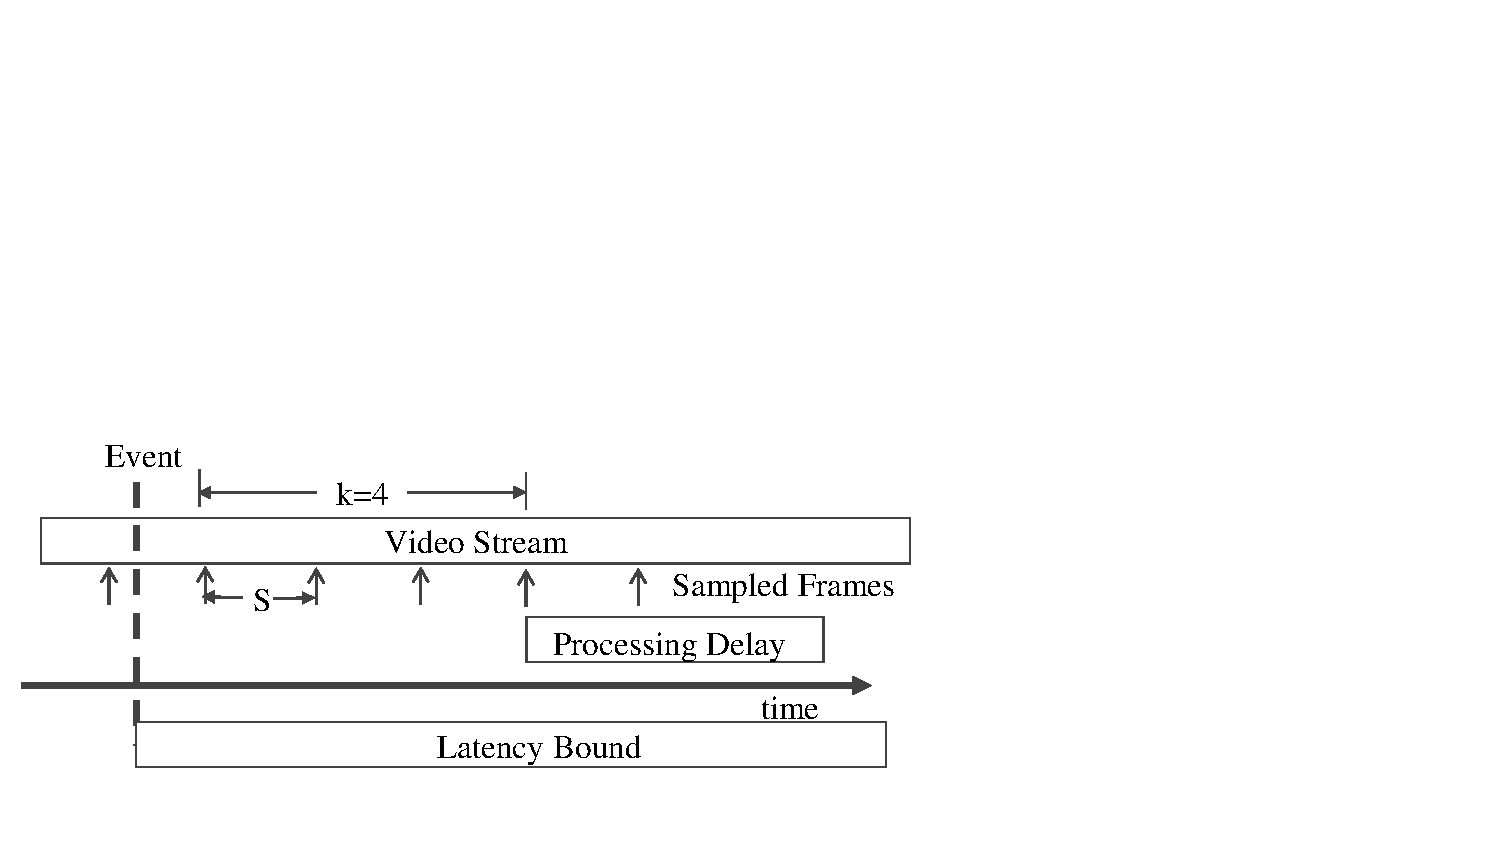
\includegraphics[width=\textwidth,trim=0em 3em 20em 15em, clip]{FIGS/fig-lego-sampling-model.pdf}
\caption{\small Dynamic Sampling Rate for LEGO}
\label{fig:lego-sampling-model}
\end{figure}

We use the LEGO application from Section~\ref{sec:example-apps} to show the
effectiveness of adaptive sampling. By default, the LEGO application runs at
active phase. The application enters passive phases immediately following the
delivery of an instruction, since the user is going to take a few seconds
searching and assembling LEGO blocks. The length and sampling rate of a passive
phase is provided by the application to the framework. We provide the following
system model as an example of what can be provided. We collect five LEGO traces
with 13739 frames as our evaluation dataset.

\textbf{Length of a Passive Phase: }
We model the time it takes to finish each step as a Gaussian distribution. We
use maximum likelihood estimation to calculate the parameters of the Guassian
model.

 
\begin{figure}
\small\centering
\begin{subfigure}{.45\linewidth}
  \centering
  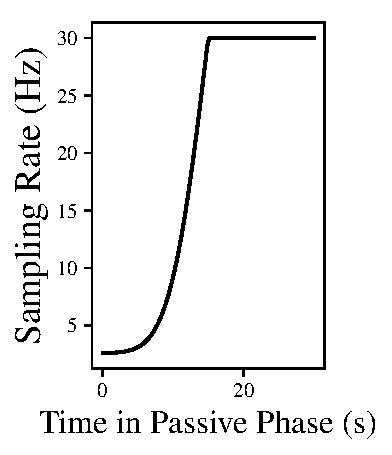
\includegraphics[width=\linewidth, trim=0em 0em 0em 0em, clip]{FIGS/fig-lego-adaptive-sr.pdf}
  {\small (a) Passive Sampling Rate}
\end{subfigure}
\begin{subfigure}{.45\linewidth}
    \centering
    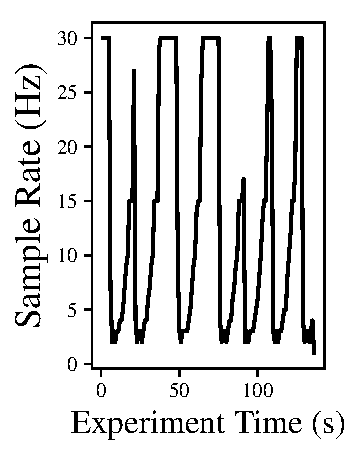
\includegraphics[width=0.92\linewidth, trim=0em 0em 0em 0em, clip]{FIGS/fig-lego-example-sr.pdf}
   {\small (b) Trace Sampling Rate}
\end{subfigure}
\caption{\small Adaptive Sampling Rate}
\label{fig:adaptive-sampling-example}
\end{figure}

\textbf{Lowest Sampling Rate in Passive Phase: }
The lowest sampling rate in passive phase still needs to meet application's
latency requirement. Figure~\ref{fig:lego-sampling-model} shows the system model
to calculate the largest sampling period S that still meets the latency bound.
In particular,
$$(k-1)S + processing\_delay \leq latency\_bound $$ $k$ represents the
cumulative number of frames an event needs to be detected in order to be
certain an event actually occurred. The LEGO application empirically sets this
value to be 5. 

\textbf{Adaptation Algorithm: }
At the start of a passive phase, we set the sampling rate to the
minimum calculated above.  As time progresses, we gradually increase
the sampling rate.  The idea behind this is that the initial low
sampling rates do not provide good latency, but this is acceptable, as
the likelihood of an event is low.  As the likelihood increases (based
on the Gaussian distribution described earlier), we increase sampling
rate to decrease latency when events are likely.
Figure~\ref{fig:adaptive-sampling-example}(a) shows the sampling rate
adaptation our system employs during a passive phase.
The sampling rate is calculated as $$sr = \\
%
 min\_sr + \alpha * (max\_sr - min\_sr) * cdf\_Gaussian(t)$$ 
%
$sr$ is the sampling rate. $t$ is the time after an instruction has been given. $\alpha$ is
a recovery factor which determines how quickly the sampling rate
rebounds to active phase rate. 


Figure~\ref{fig:adaptive-sampling-example}(b) shows the sampling rate
for a trace as the application runs. The video captures a user doing 7
steps of a LEGO assembly task. Each drop in sampling rate happens
after an instruction has been delivered to the user.
Table~\ref{tab:adaptive-sample-eval} shows the percentage of frames
sampled and guidance latency comparing adaptive sampling with naive
sampling at half frequency. Our adaptive sampling scheme requires
processing fewer frames while achieving a lower guidance latency.

\begin{table}[]
\small\centering
\begin{tabular}{|c|c|c|}
\hline
Trace  & \begin{tabular}[c]{@{}c@{}}Sample\\ Half Freq\end{tabular} & \begin{tabular}[c]{@{}c@{}}Adaptive\\ Sampling\end{tabular} \\ \hline
1 & 50\%          & 25\%              \\ \hline
2 & 50\%          & 28\%              \\ \hline
3 & 50\%          & 30\%              \\ \hline
4 & 50\%          & 30\%              \\ \hline
5 & 50\%          & 43\%              \\ \hline
\end{tabular}\\[0.1in]
{\small (a) Percentage of Frames Sampled}\\[0.2in]

\begin{tabular}{|c|c|}
\hline
                                                            & \begin{tabular}[c]{@{}c@{}}Guidance Delay \\ (frames$\pm$stddev)\end{tabular}
                                                            \\ \hline
\begin{tabular}[c]{@{}c@{}}Sample Half Freq\end{tabular}      & 7.6 $\pm$ 6.9                                                                  \\ \hline
\begin{tabular}[c]{@{}c@{}}Adaptive Sampling\end{tabular} &  5.9 $\pm$ 8.2                                                                  \\ \hline
% \begin{tabular}[c]{@{}c@{}}Theoretical Minimum\end{tabular} &  ?? $$                                                                  \\ \hline
\end{tabular}\\[0.1in]
{\small (b) Guidance Latency}\\[0.1in]
\caption{\small Frames Sampled and Guidance Latency}
\label{tab:adaptive-sample-eval}
\vspace{-0.2in}
\end{table}